\documentclass{article} 
\usepackage{listings}
\usepackage{graphicx}
\usepackage{subfig}
\usepackage{multirow}
\usepackage{float}
\usepackage{algorithm}
\usepackage{algpseudocode}
\usepackage{amsmath}

\newenvironment{algocolor}{%
   \setlength{\parindent}{0pt}
   \itshape
   \color{blue}
}{}

\lstset
{ %Formatting for code in appendix
    language=Python,
    %basicstyle=\footnotesize,
    numbers=left,
    stepnumber=1,
    showstringspaces=true,
    tabsize=4,
    breaklines=true,
    breakatwhitespace=false,
}

\title{AI 534 IA3 Report}
\author{Rishab Balasubramanian}
\date{}

\begin{document}
\maketitle

\textbf{1.a.} We can see that the curves in Fig.\ref{fig:Perceptron} for online perceptron is relatively more oscillatory, compared to that of the average perceptron. We can attribute this to the fact that the online perceptron adds $w \leftarrow y_{i}x_{i}$ directly after each misclassified training example. In comparison, the average perceptron only adds a fraction of this $ w \leftarrow w + z$, where $z = 0$ if the training example is correctly classified, and $z = y_{i}x_{i}/(s+1)$ if not. Thus we see that the change in weights of the average perceptron is much smaller than that of the online perceptron, and as we keep iterating through the set of training examples the denominator of the update function keeps increasing (i.e, the change in w decreases) in the case of average perceptron. This explains the smoother curves from average perceptron, compared to the oscillatory ones from online perceptron.\\

\textbf{b.} \\
Online Perceptron : Best Validation Accuracy - $76.6\%$, Iteration number - $48$\\
Average Perceptron : Best Validation Accuracy - $79.19\%$, Iteration number - $1$\\

As we can see, the online perceptron is more sensitive to the stopping point. This is because of how the weights are constantly changing in the case of online perceptron, which causes large variations in prediction accuracies in comparison to the average percpetron, where the change in weights become negligible as the number of iterations increases. As a result, I feel average perceptron should generally always give better results than online perceptron. Thus, vanilla perceptron is rarely used for experiments, and is replace with average perceptron. One drawback of the average perceptron is that it gives more weight to data which appears earlier, than those that appear later in the dataset. As a result shuffling the data leads to better results as shown in Fig.\ref{fig:ShuffledPerceptron}. We see that the best accuracies obtained after randomizing data order are:\\ \\
Online Perceptron : Best Validation Accuracy - $78.1\%$, Iteration number - $45$\\
Average Perceptron : Best Validation Accuracy - $79.45\%$, Iteration number - $1$

\begin{figure}[H]
    \centering
    \subfloat[\centering Online Perceptron]{{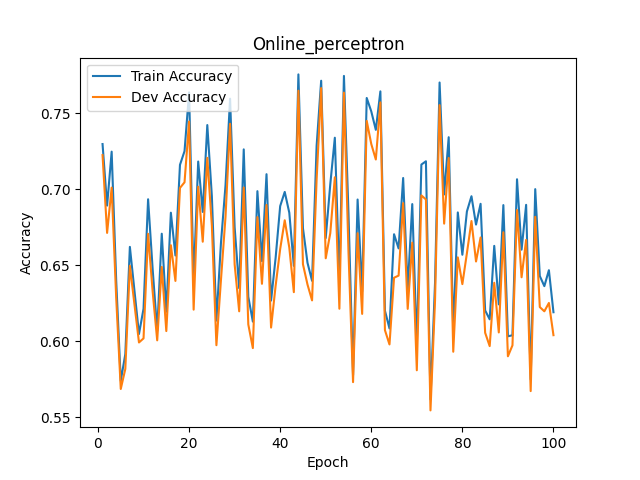
\includegraphics[width=0.33\textwidth, height=4cm]{./figs/Online_perceptron.png} }}
    \subfloat[\centering Average Perceptron]{{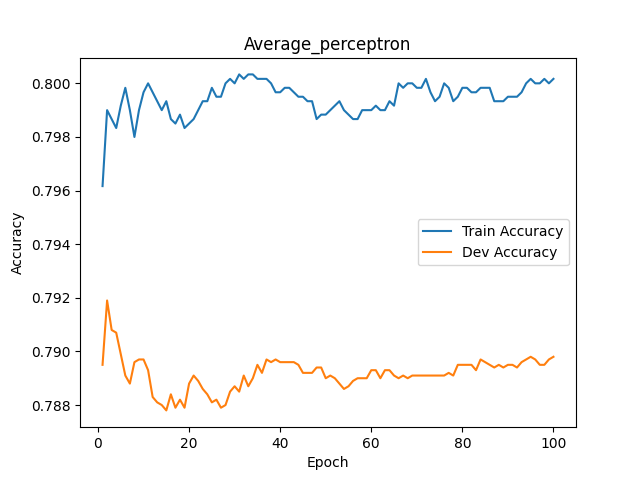
\includegraphics[width=0.33\textwidth, height=4cm]{./figs/Average_perceptron.png} }}
    \subfloat[\centering Online vs Average Perceptron]{{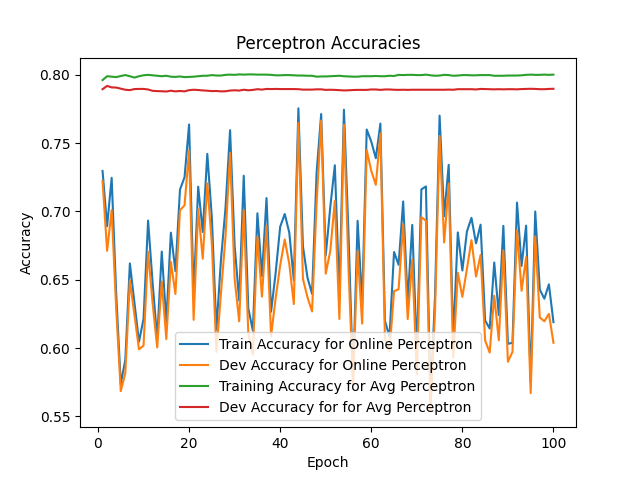
\includegraphics[width=0.33\textwidth, height=4cm]{./figs/Perceptron.png} }}\\
\caption{Training and Validation Accuracy for Perceptron Algorithm}
    \label{fig:Perceptron}%
\end{figure}


\begin{figure}[H]
    \centering
    \subfloat[\centering Online Perceptron]{{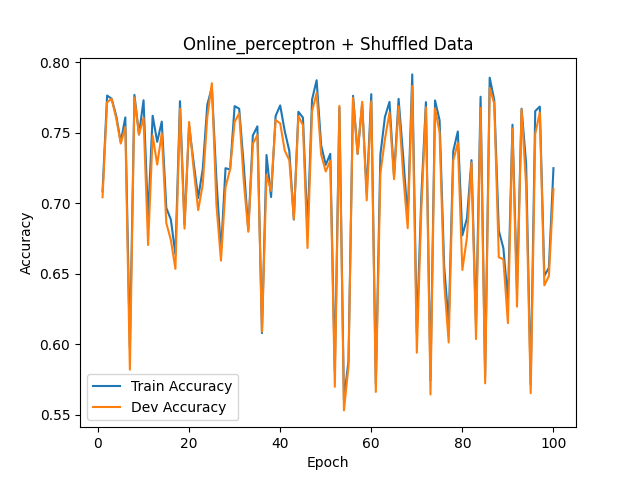
\includegraphics[width=0.33\textwidth, height=4cm]{./figs/Online_perceptron_Random.png} }}
    \subfloat[\centering Average Perceptron]{{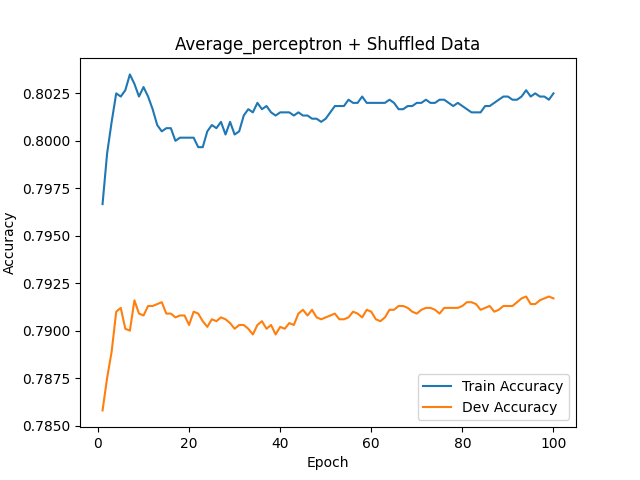
\includegraphics[width=0.33\textwidth, height=4cm]{./figs/Average_perceptron_Random.png} }}
    \subfloat[\centering Online vs Average Perceptron]{{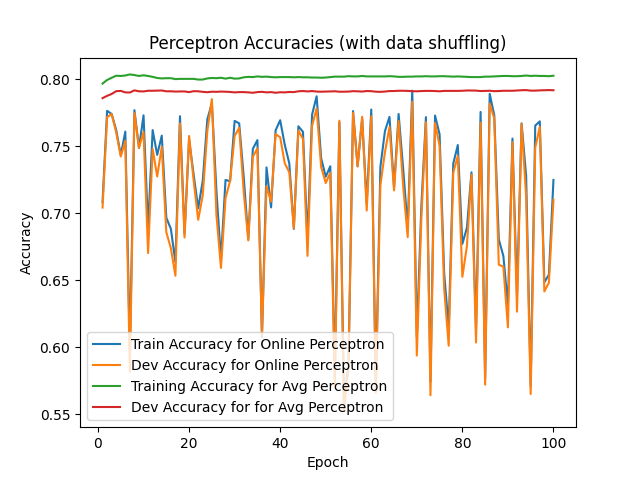
\includegraphics[width=0.33\textwidth, height=4cm]{./figs/Perceptron_Random.png} }}\\
\caption{Training and Validation Accuracy for Perceptron Algorithm with Data Shuffling}
    \label{fig:ShuffledPerceptron}%
\end{figure}
\newpage


\textbf{2a.a} As $p$ increases, the number of features increases as well due to the increase in dimensionality. As a result we see that for higher values of $p$ the model overfits (i.e the training accuracy is lower than the validation accuracy, and training accuracy keeps increasing, while validation accuracy is almost constant), which is highlighted in Fig.\ref{fig:Kernalized_perceptron}. We see that for $p=1(2)$, the training and validation accuracies are similar, and follow a similar oscillatory(upward) trend. For the other values of $p$, we see that the training accuracy is significantly larger than the validation accuracy and keeps increasing, implying the model overfits to the training data. We can attribute this to the extra features introduced by increasing dimensions, which results in overfitting (similar to how the model overfits with a higher order polynomials for linear regression).\\

\textbf{b} Table.\ref{table:Accuracy} shows the best training and vaidation accuacies for all values of $p$. $p=1$ produces the best validation accuracy. As the value of $p$ increases, we see that the model overfits, and as a result the training accuracy increases, while validation accuracy slowly decreases/remains constant (highlighted clearly for $p=5$). 

\begin{figure}[H]
    \centering
    \subfloat[\centering p=1]{{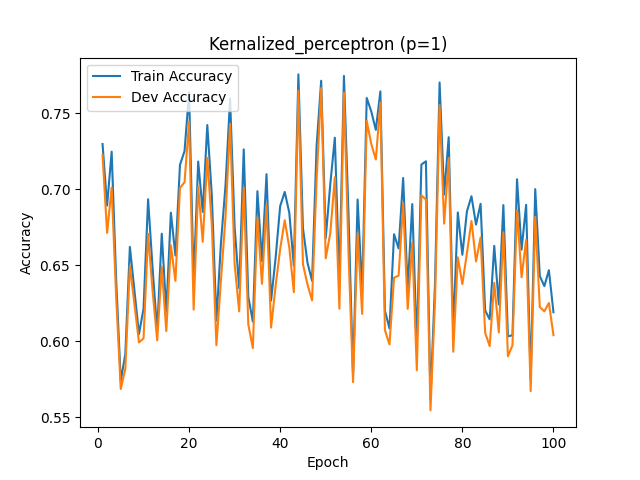
\includegraphics[width=0.5\textwidth, height=4.25cm]{./figs/Kernalized_perceptron (p=1).png} }}
    \subfloat[\centering p=2]{{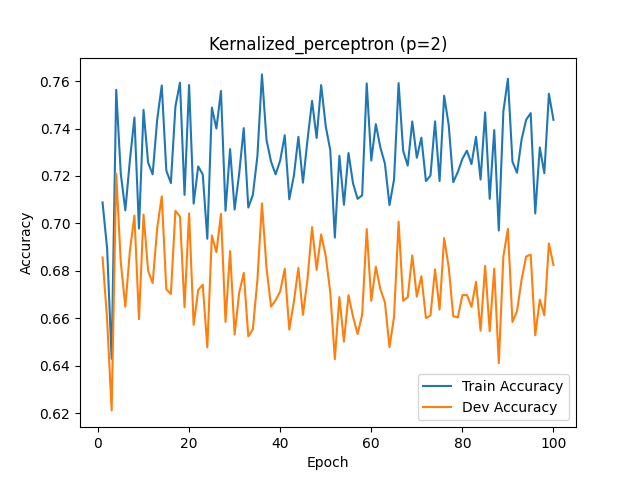
\includegraphics[width=0.5\textwidth, height=4.25cm]{./figs/Kernalized_perceptron (p=2).png} }}\\
    \subfloat[\centering p=3]{{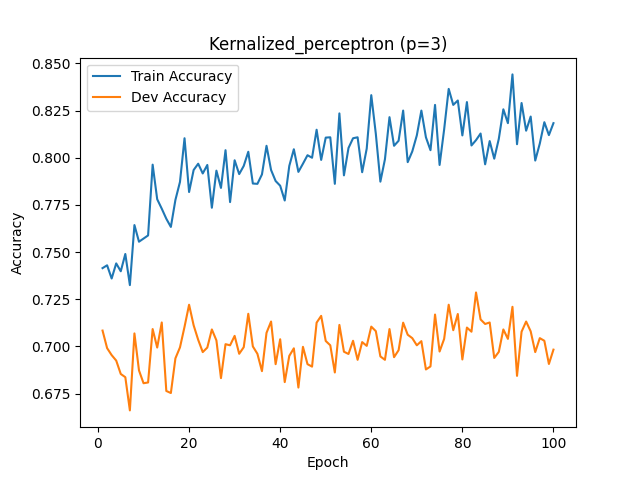
\includegraphics[width=0.33\textwidth, height=4.25cm]{./figs/Kernalized_perceptron (p=3).png} }}
    \subfloat[\centering p=4]{{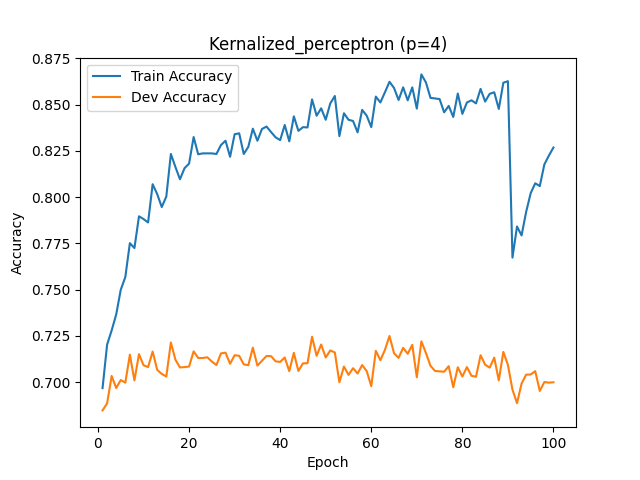
\includegraphics[width=0.33\textwidth, height=4.25cm]{./figs/Kernalized_perceptron (p=4).png} }}
    \subfloat[\centering p=5]{{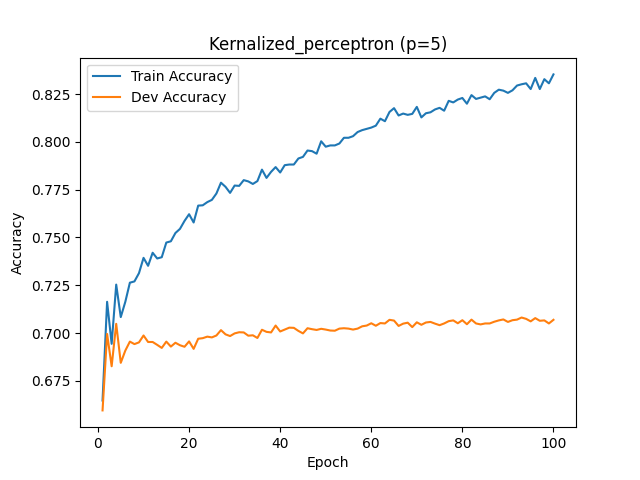
\includegraphics[width=0.33\textwidth, height=4.25cm]{./figs/Kernalized_perceptron (p=5).png} }}\\
    \caption{Kernelized Perceptron for different values of p}
    \label{fig:Kernalized_perceptron}%
\end{figure}



\begin{table}
\caption{Best Accuracies for different values of $p$ for Kernelized Perceptron}
\begin{tabular}{ |p{4cm}||p{4cm}||p{4cm}|  }
 \hline  
 \multicolumn{3}{|c|}{$p=1$} \\
 \hline
  & Accuracy & Epoch\\
 \hline
Training & $77.54\%$ & $43$\\
Validation & $76.6\%$ & $48$\\
\hline 
 \multicolumn{3}{|c|}{$p=2$} \\
 \hline
  & Accuracy & Epoch\\
 \hline
Training & $76.28\%$ & $35$\\
Validation & $72.09\%$ & $3$\\
\hline 
 \multicolumn{3}{|c|}{$p=3$} \\
 \hline
  & Accuracy & Epoch\\
 \hline
Training & $84.41\%$ & $90$\\
Validation & $72.86\%$ & $82$\\
\hline 
 \multicolumn{3}{|c|}{$p=4$} \\
 \hline
  & Accuracy & Epoch\\
 \hline
Training & $86.63\%$ & $70$\\
Validation & $72.49\%$ & $63$\\
\hline 
 \multicolumn{3}{|c|}{$p=5$} \\
 \hline
  & Accuracy & Epoch\\
 \hline
Training & $83.53\%$ & $99$\\
Validation & $70.80\%$ & $92$\\
 \hline
\end{tabular}
\label{table:Accuracy}
\end{table}
\vspace{\baselineskip}


\textbf{c.} Fig.\ref{fig:Runtime}a. shows the runtime of the Online Kernelized Perceptron Algorithm. The asymptotic time complexity of the algorithm is:
\begin{itemize}
\item Let the maximum number of iterations be $m$, the dimension of the data $d$, and number of examples $n$.
\item Generating the kernel the matrix takes $O(n^{2}d)$ time
\item We train for $m$ iterations
\item Each time, we iterate through the data set, and predict the output for each example, which takes $O(nd)$ time.
\item Therefore training in total takes $O(mnd)$ time, and including the time for kernelizing, we get $O(n^{2}d + mnd)$.
\item As $n>>m$ and $n>>d$, we can approximate this to $O(n^{3})$ time.
\end{itemize}

We see that $n^{3}$ acts as an upperbound for the runtime of the algorithm for larger values of $n$.


\begin{figure}[H]
	\centering
    \subfloat[\centering Online]{{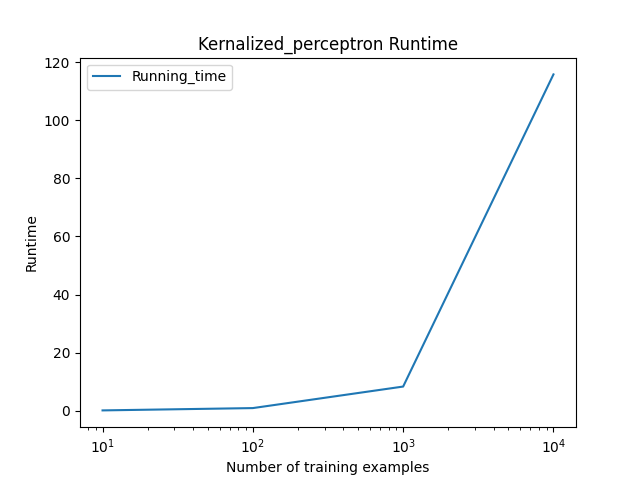
\includegraphics[width=0.45\textwidth, height=4.5cm]{./figs/part2a_runtime.png} }}\label{fig:a}
    \subfloat[\centering Batch]{{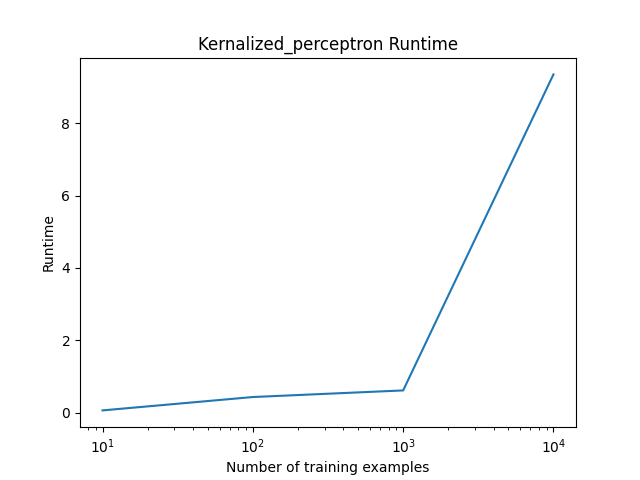
\includegraphics[width=0.45\textwidth, height=4.5cm]{./figs/part2b_runtime.png} }}\label{fig:b}\\
    \caption{Runtime for Kernelized Perceptron}
    \label{fig:Runtime}%
\end{figure}


\textbf{2b.a.} 1. Fig.\ref{fig:Batch_KP} shows the plot for batch kernel perceptron. The batch kernel perceptron seems to oscillate more than the online kernel perceptron. This is because we update the $\alpha$ simultaneously after going throught the entire training data. Consider a scenario where examples in the training data, $x_{1}$ and $x_{2}$ are incorrectly labelled with the weights ($w_{t}$) at iteration $t$. In the online case, changing the weights after detecting misclassification of $x_{1}$ could possibly ensure that the next example $x_{2}$ is correctly classified. However in the batch update, as the weights are updated simultaneously, both examples $x_{1}$, and $x_{2}$ contribute to weight updates, thus causing larger changes in the $\alpha$ resulting in oscillations.\\

2. Having a learning rate would simply rescale the weights, but would not affect the decision boundary itself. If $w^{T}x > 0$, then for any positive value $c$, $cw^{T}x > 0$ is true. However, the algorithm would be affected if the learning rate is negative. \\

\textbf{b.} Algorithm.\ref{alg:algo} shows the algorithm for batch kernelized perceptron and Fig. \ref{fig:Runtime}b shows the corresponding running time. The batch perceptron, would again have $O(n^{2}d)$ time for generating the kernel matrices ($n$ = number of training examples, $d$ = dimension of the data). For each training iteration, the algorithm would have to multiply each row of the kernel matrix with $\alpha$, which takes $O(n^{2})$ time. Thus the total time is $O(n^{2}d + n^{2}m) = O(n^{3})$. We see that $O(n^{3})$ provides a satisfactory upper bound on the running time of the algorithm. We however notice a significant speed up of our code, although no major changes have been made. This can be attributed to the use of python libraries (numpy), which use a effiecint static programming (C/C++) language to perform these computations, which results in the significant speed up.\\

\begin{algorithm}
\caption{Batch Kernalized Perceptron Algorithm}\label{alg:algo}
\hspace*{\algorithmicindent} \textbf{Input} $\{(\mathbf{x}_{i}, y_{i})_{i=1}^{N}\}$(for both training and dev data) $, maxiter, \kappa$(kernel function) \\
\hspace*{\algorithmicindent} \textbf{Output} $\boldsymbol\alpha = [ \alpha_{1}, \alpha_{2}, \cdots, \alpha_{N}]^{T}$ 
\begin{algorithmic}[1]
	\State $\alpha_{i} \leftarrow 0$ for $i = 1, \cdots, N$
	\For {$i=1, \cdots N,\: j=1, \cdots, N$}
		\State $K(i, j) = \kappa(x_{i}, x_{j}) \Rightarrow K_{train} = (train*train^{T})^{p}, K_{dev} = (dev*train^{T})^{p}$  where $train$ is the training data, $dev$ is the dev data 
		\State (\textit{This can be done by multiplying the training data and its transpose giving a (6000*6000) matrix for the training kernel, and multiplying the validation data and training data to give (10000*6000) matrix for the validation kernel})
	\EndFor
	\While {$iter < maxiter$}
		\State $\boldsymbol\alpha = \boldsymbol\alpha + K_{train} \boldsymbol\alpha \mathbf{y_{train}}$
	\EndWhile
\end{algorithmic}
\end{algorithm}

\begin{figure}[H]
	\centering
    \subfloat{{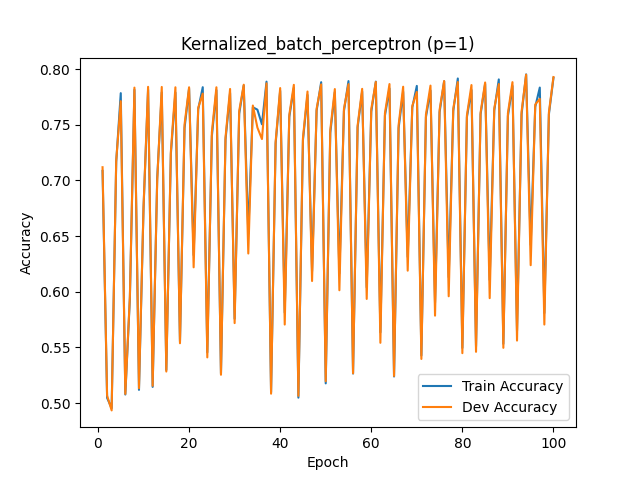
\includegraphics[width=1\textwidth, height=7cm]{./figs/Kernalized_batch_perceptron (p=1).png} }}
    \caption{Batch Kernelized Perceptron}
    \label{fig:Batch_KP}%
\end{figure}

\end{document}